\documentclass[a4paper,12pt]{article}

% Pakete
\usepackage[ngerman]{babel}
\usepackage[utf8]{inputenc}
\usepackage[T1]{fontenc}
\usepackage{graphicx}
\usepackage{amsmath}
\usepackage{fp}
\usepackage{siunitx}
\usepackage{spreadtab}
\usepackage{booktabs}
\usepackage{geometry}
\usepackage{tabularx}
\usepackage{caption}
\usepackage{float}
\usepackage[colorlinks=true,linkcolor=black]{hyperref}
\usepackage{pdfpages}
\geometry{margin=2.5cm}
\sisetup{locale=DE}

% Titelinformationen
\title{\textbf{\underline{Physikpraktikum für Mediziner}} \\[2em]
\Large \textbf{Versuch 16: Temperaturmessung}}

\author{
    Thea Lee und David N. Vinu \\[0.5em]
    \makebox[\textwidth][s]{%
        17. März 2026 \hfill Assistent: Felix Exner \hfill Messplatz: B \hfill Gruppe: 4b
    }
}

\date{}

\begin{document}
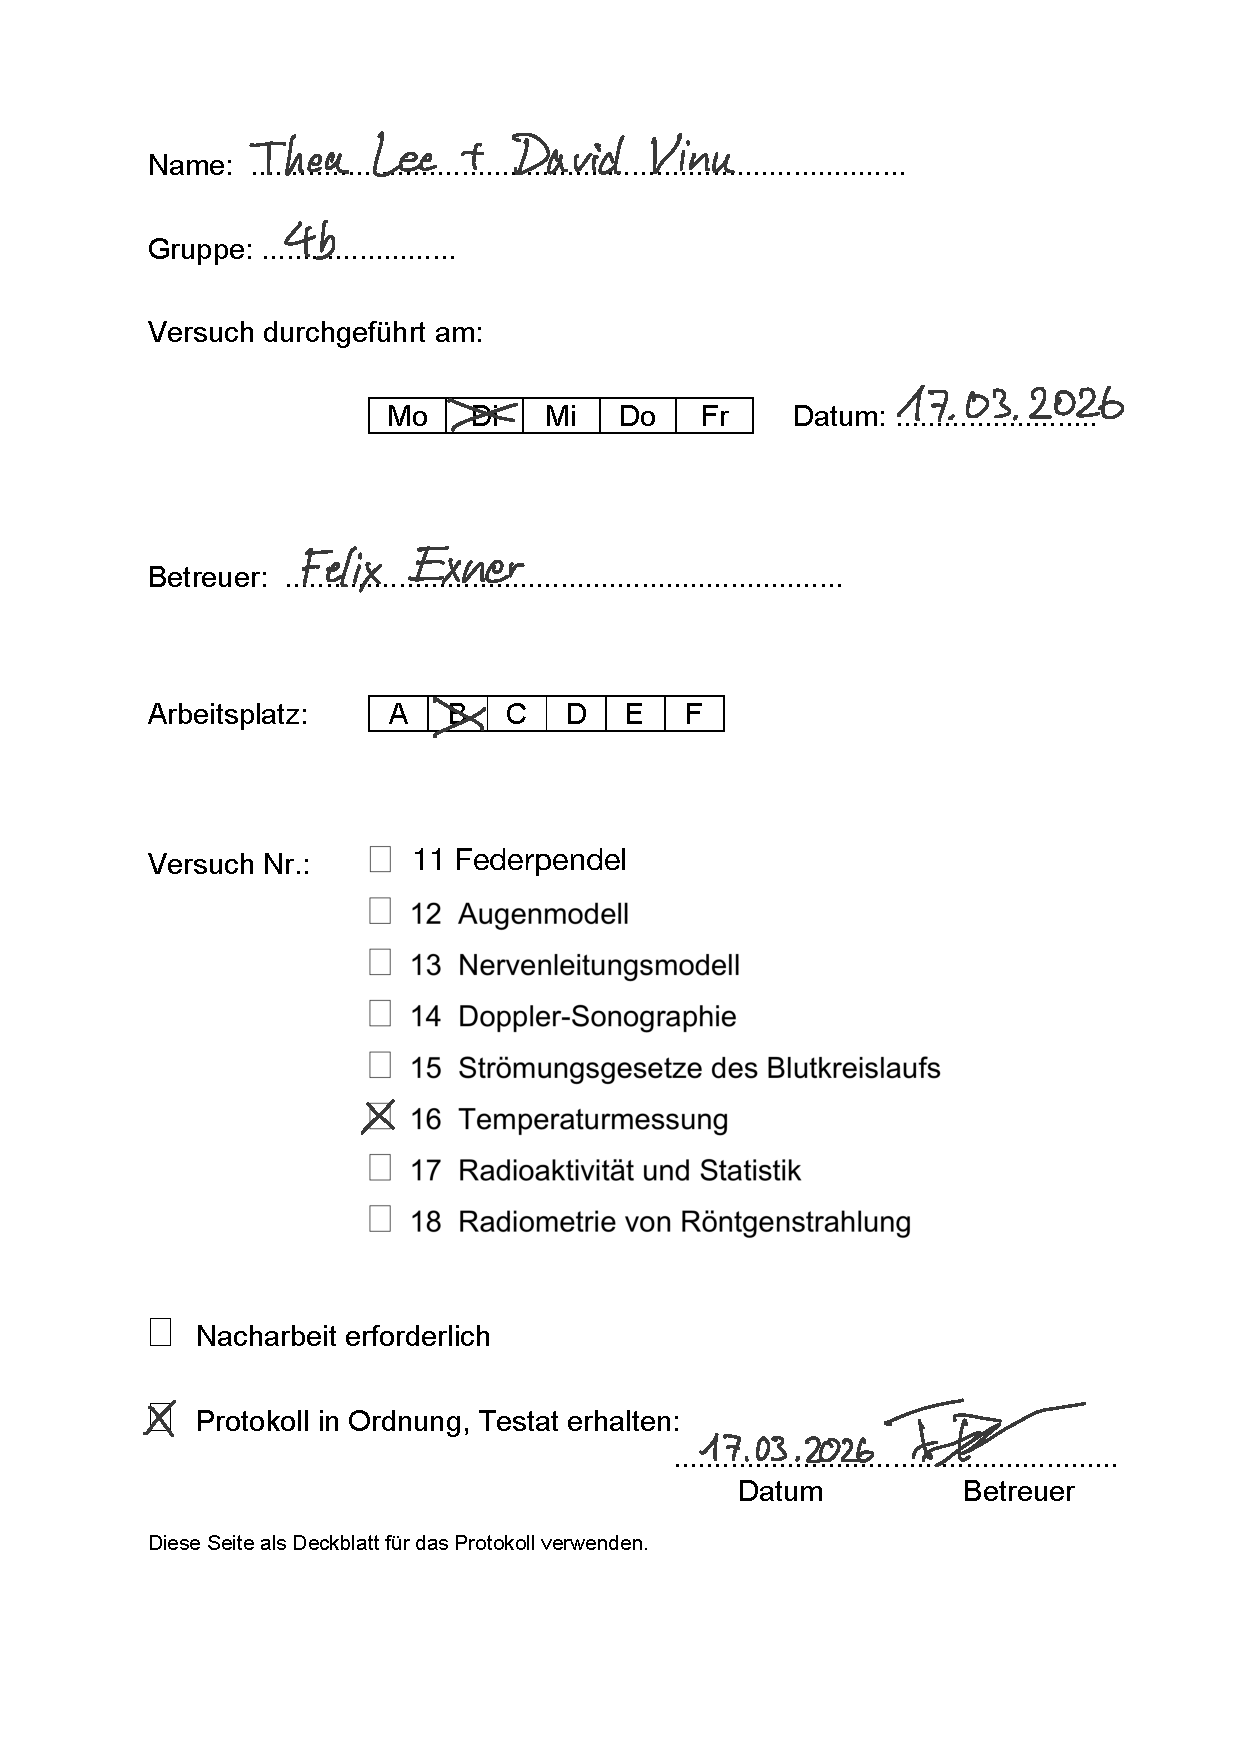
\includepdf[pages=1,scale=1,frame=false]{Copy of Protokolldeckblatt (2015) +11.pdf}
\maketitle
\tableofcontents
\newpage

\section{Grundlagen}
\subsection{Aufgabenstellung}
- Aufgabe 1: Eichung der Thermometer bei \SI{0}{\celsius} \\
- Aufgabe 2: Temperaturmessung bis \( T = \SI{100}{\celsius} \) \\
- Aufgabe 3: Messung von sehr hohen Temperaturen mit dem PtRh-Thermoelement

\subsection{Skizzen Versuchsaufbau}
\begin{figure}[H]
    \centering
    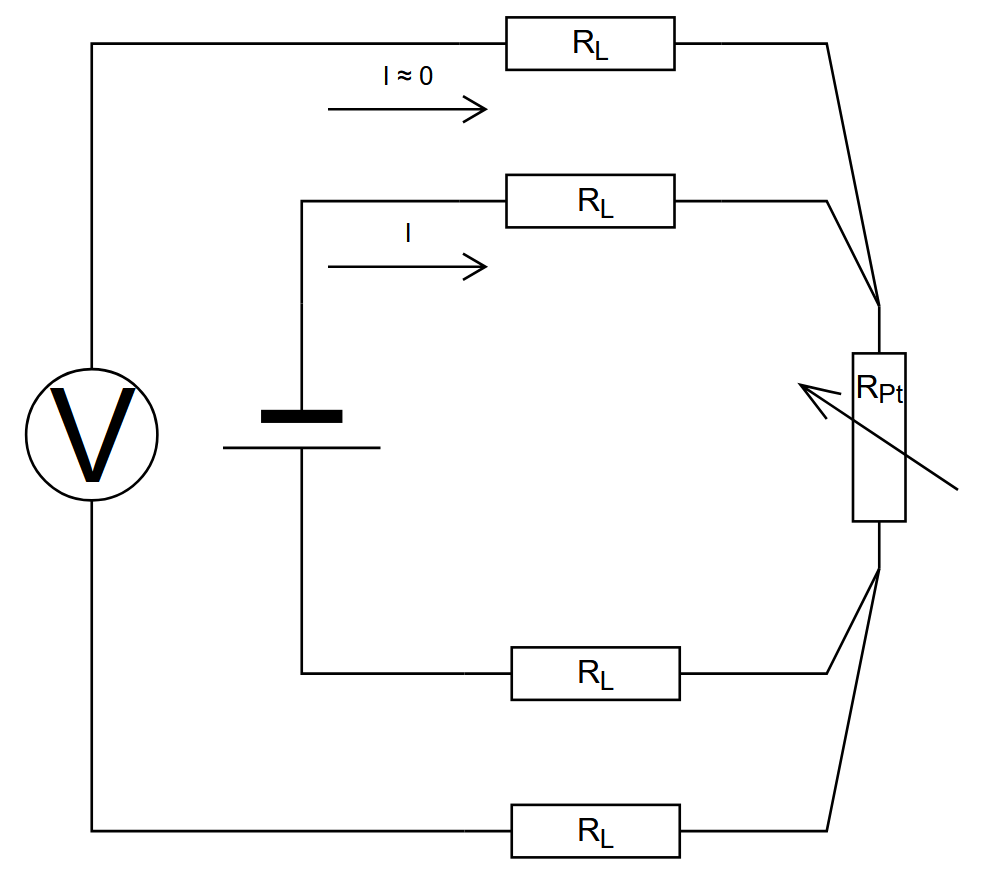
\includegraphics[width=1\linewidth]{Screenshot 2026-03-22 123212.png}
    \begin{tabular}{rl}
    $R_\mathrm{L}$: & Leitungswiderstand \\
    $R_\mathrm{Pt}$: & Temperaturabhängiger Widerstand \\
    \end{tabular}
    \caption{Vierleiterschaltung zur Widerstandsmessung}
    \label{fig:vierleiter}
\end{figure}

\begin{figure}[H]
    \centering
    \begin{minipage}{0.56\linewidth}
        \centering
        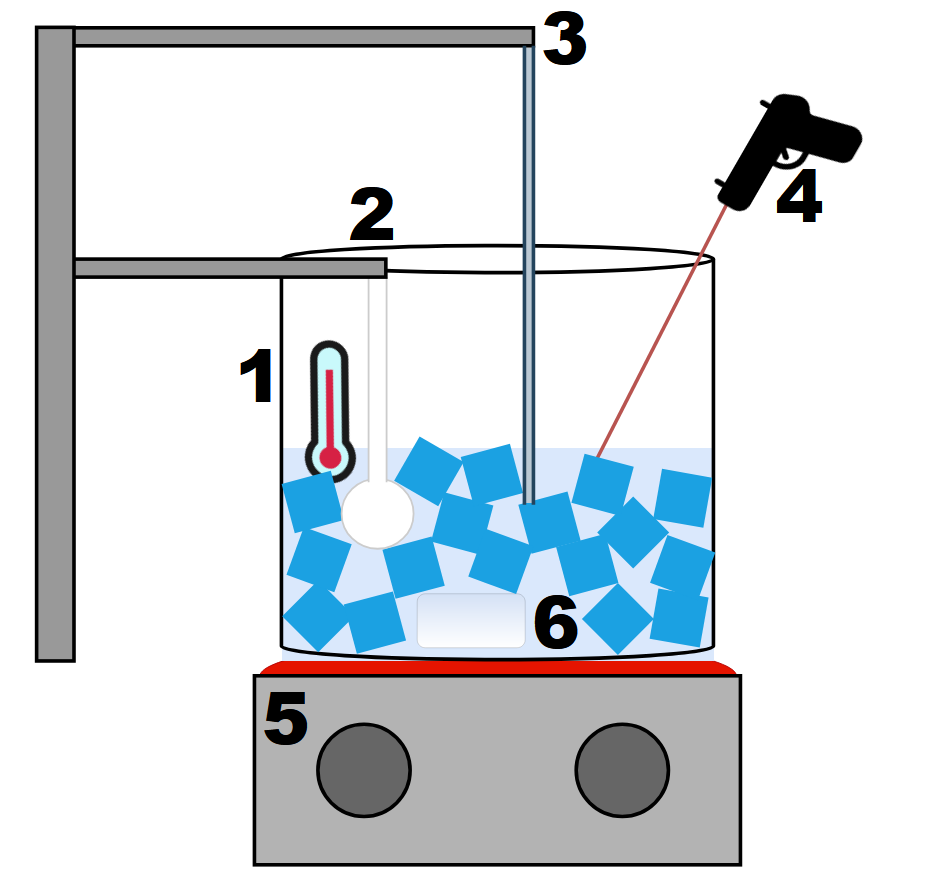
\includegraphics[width=\linewidth]{Screenshot 2026-03-22 105709.png}
        \captionof{figure}{Eichung und Temperaturmessung von \SI{0}{\celsius} bis \SI{100}{\celsius}}
        \label{fig:temp-messung}
    \end{minipage}
    \hfill
    \begin{minipage}{0.4\linewidth}
        \centering
        \begin{tabular}{rl}
            Abb. 2 \\
            1: & Flüssigkeitsthermometer \\
            2: & Gasthermometer \\
            3: & Pt100-Widerstandsthermometer \\
            4: & Pyrometer \\
            5: & Heizplatte \\
            6: & Rührfisch \\\\
        \end{tabular}
        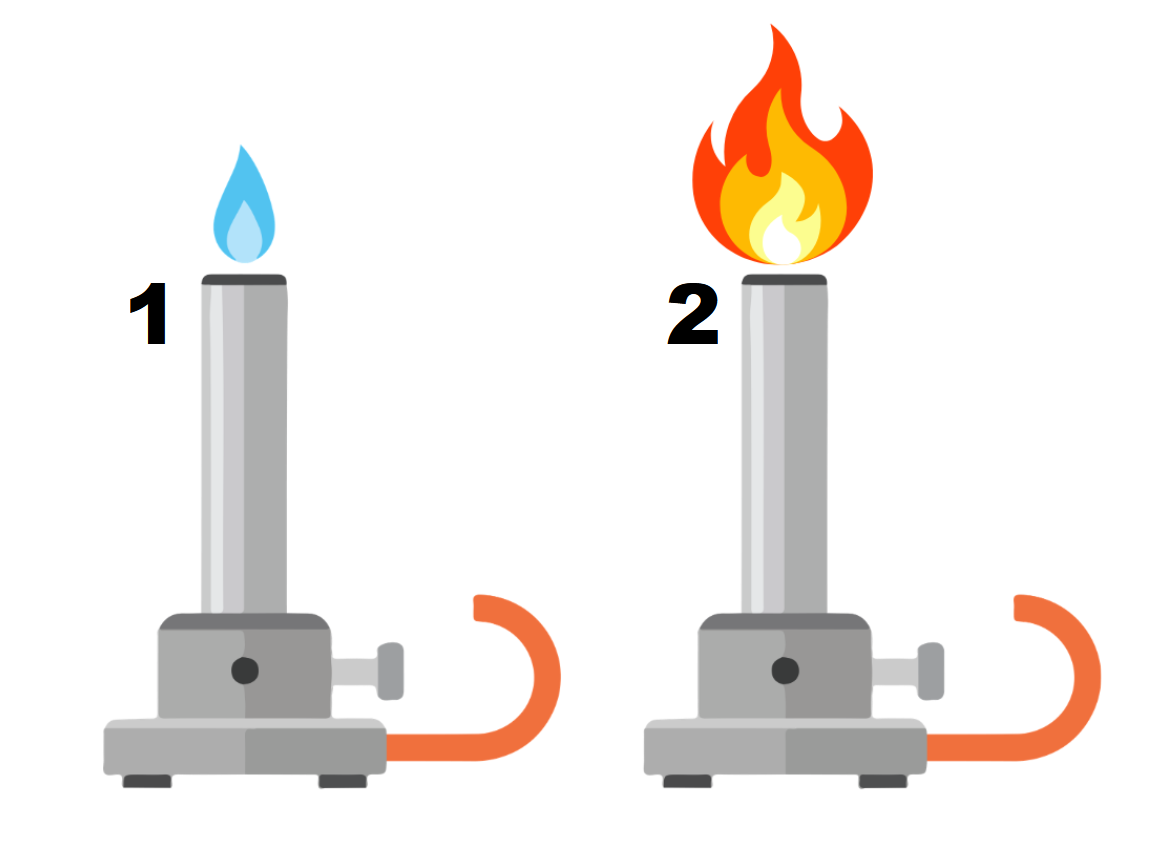
\includegraphics[width=\linewidth]{Screenshot 2026-03-22 131246.png}
        \begin{tabular}{rl}
            1: & Vollständige Verbrennung \\
            2: & Unvollständige Verbrennung
        \end{tabular}
        \captionof{figure}{Flammen der vollständigen und unvollständigen Verbrennung}
        \label{fig:bunsenbrenner}
    \end{minipage}
\end{figure}

\subsection{Vorausgesetzte Formeln}

\paragraph{Ideales Gasgesetz}
\begin{equation}
    pV = nRT \quad \Rightarrow \quad T \propto p
\end{equation}

\paragraph{Gesetz von Amontons}
\begin{equation}
    p \propto T \quad \text{für } V = \text{const.},\ n = \text{const.}
\end{equation}

\paragraph{Thermoelement (Seebeck-Effekt)}
\begin{equation}
    U_{\text{th}} = K(T_1 - T_2)
\end{equation}

\paragraph{Pt100-Widerstand in Abhängigkeit von T}
\begin{equation}
    R(T) = R_0 \bigl(1 + A T + B T^2\bigr)
\end{equation}
mit
\begin{equation*}
\begin{gathered}
    R_0 = 100~\si{\ohm} \\
    A = 3{,}9083 \times 10^{-3}~\si{\per\celsius} \\
    B = -5{,}775 \times 10^{-7}~\si{\celsius^{-2}} \\
\end{gathered}
\end{equation*}

\paragraph{Ohmsches Gesetz}
\begin{equation}
    U = R \cdot I
\end{equation}

\paragraph{Plancksches Strahlungsgesetz}
\begin{equation}
M_\lambda(\lambda,T) \, \mathrm{d}A \, \mathrm{d}\lambda = \frac{2\pi h c^2}{\lambda^5} \frac{1}{e^{\frac{hc}{\lambda k T}}-1} \, \mathrm{d}A \, \mathrm{d}\lambda
\end{equation}

\paragraph{Stefan-Boltzmann-Gesetz}
\begin{equation}
P = \epsilon(T) \sigma A T^4
\end{equation}

\paragraph{Druckumrechnung}
\begin{equation}
p_\text{NB} = p_\text{gem} \frac{1013{,}25~\text{hPa}}{p_\text{LD}}
\end{equation}

\subsection{Abgewandelte Formeln}
\subsubsection*{Widerstandsthermometer}
Um die Temperatur in Abhängigkeit des Widerstands darzustellen, muss die Umkehrfunktion gebildet werden. Dafür wird zunächst nach T umgeformt. Da die Polynome der Funktion verschiedene Exponenten von T enthalten, ist eine quadratische Ergänzung notwendig.

\begin{equation*}
\begin{aligned}
\Rightarrow R&=R_{0}\left(1+A T+B T^{2}\right) 
&| : R_{0} 
\\ 
\frac{R}{R_{0}}&=1+A T+B T^{2} 
\\ 
\frac{R}{R_{0}}&=1+A T+B T^{2}
&| : B
\\ 
\frac{R}{R_{0} B}&=\frac{1}{B}+\frac{A}{B} \cdot T+T^{2} 
\\ 
\Rightarrow \frac{R}{R_{0} \cdot B}&=\frac{1}{B}+2\left(\frac{A}{2 B}\right) \cdot T+T^{2}+\left(\frac{A}{2 B}\right)^{2}-\left(\frac{A}{2 B}\right)^{2} 
&\phantom{|}
\\ 
\frac{R}{R_{0} \cdot B}&=T^{2}+2\left(\frac{A}{2 B}\right) \cdot T+\left(\frac{A}{2 B}\right)^{2}-\left(\frac{A}{2 B}\right)^{2}+\frac{1}{B} 
&\phantom{|}
\\ 
\frac{R}{R_{0} \cdot B}&=
 \left(T+\left(\frac{A}{2 B}\right)\right)^{2}-\left(\frac{A}{2 B}\right)^{2}+\frac{1}{B}
 &| +\left(\frac{A}{2 B}\right)^{2} -\frac{1}{B} 
\\ 
\frac{R}{R_{0} \cdot B}+\left(\frac{A}{2 B}\right)^{2}-\frac{1}{B}&=\left(T+\left(\frac{A}{2 B}\right)^{2}-\frac{1}{B}\right)^{2} 
&| \sqrt{}
\\ 
\sqrt{\left.\frac{R}{R_{0} \cdot B}-\left\lvert\, \frac{A}{2 B}\right.\right.)^{2}+1}&=T+\frac{A}{2 B}
&| -\frac{A}{2 B} 
\\ 
\sqrt{\frac{R}{R_{0} \cdot B}+\frac{A^{2}}{4 B^{2}}-\frac{1}{B}}-\frac{A}{2 B}&=T
&\phantom{|}
\end{aligned}
\end{equation*}
\begin{equation}
\Rightarrow T(R)=\sqrt{\frac{R}{R_{0} \cdot B}+\frac{A^{2}}{4 B^{2}}-\frac{1}{B}}-\frac{A}{2 B}
\end{equation}

\subsection{Verwendete Variablen}

\begin{description}
\item[$p$] Druck
\item[$V$] Volumen 
\item[$n$] Stoffmenge
\item[$R$] Gaskonstante
\item[$T$] Temperatur
\item[$U_\mathrm{th}$] Thermospannung
\item[$K$] Seebeck-Koeffizient
\item[$T_1$] Temperatur an der Kontaktstelle der Metalle
\item[$T_2$] Temperatur an den Enden der beiden Metalle
\item[$R(T)$] Widerstand bei $T$
\item[$R_0$] Nennwiderstand bei $0^\circ$C
\item[$A,B$] Pt100-Koeffizienten
\item[$U$] Spannung
\item[$I$] Stromstärke
\item[$\lambda$] Wellenlänge
\item[$M_\lambda$] Strahlungsleistung
\item[$dA$] infinitesimales Flächenelement 
\item[$h$] Plancksches Wirkungsquantum
\item[$c$] Lichtgeschwindigkeit
\item[$k$] Boltzmann-Konstante
\item[$P$] Strahlungsleistung
\item[$\epsilon(T)$] Emissivität
\item[$\sigma$] Stefan-Boltzmann-Konstante
\item[$A$] Fläche
\item[$p_\text{NB}$] Normbarometerdruck
\item[$p_\text{gem}$] gemessener Druck
\item[$p_\text{LD}$] Luftdruck
\end{description}

\subsection{Messverfahren}

\begin{enumerate}
    \item Eine Vierleiterschaltung wird zur Inbetriebnahme des Pt-100-Widerstandsthermometers aufgebaut. Anschließend werden in einem Becherglas, welches zur Hälfte mit klein zerstoßenem Eis und Wasser gefüllt ist, der Druck des Gasthermometers, die Spannung am Pt100-Widerstandsthermometer sowie die Temperaturanzeige des Pyrometers aufgenommen. 
    (s. Abb.~\ref{fig:vierleiter}, Seite~\pageref{fig:vierleiter})
    \item Der Versuchsaufbau aus 1. bleibt erhalten und wird um ein Flüssigkeitsthermometer ergänzt. Nun werden Temperaturwerte in Abständen von \SI{10}{\celsius} mithilfe der vier Thermometer gemessen und protokolliert. Der Temperaturanstieg wird mithilfe der Heizplatte bewerkstelligt und eine möglichst homogene Temperaturverteilung wird durch einen Rührfisch gewährleistet. Dieser Vorgang wird bis zum Siedepunkt des Wassers fortgef\"uhrt. Weiterhin wird der Luftdruck am Barometer abgelesen und notiert.
    (s. Abb.~\ref{fig:temp-messung}, Seite~\pageref{fig:temp-messung})
    \item Zur Messung hoher Temperaturen wird ein PtRh-Thermoelement in die Flamme eines Bunsenbrenners gehalten. Dabei werden die Thermospannungen an verschiedenen Positionen in der Flamme sowohl bei starker als auch bei schwacher Luftzufuhr aufgenommen.
    (s. Abb.~\ref{fig:bunsenbrenner}, Seite~\pageref{fig:bunsenbrenner})
\end{enumerate}

\section{Messprotokoll}
\sisetup{locale = DE, table-number-alignment = center}
\subsection{Temperaturmessungen am Becherglas}

\begin{table}[H]
\centering
\sisetup{
  locale=DE,
  uncertainty-mode=separate, % ± vor Unsicherheit
  separate-uncertainty=true, % separate Spalte
  table-number-alignment=center
}
\begin{tabular}{S[table-format=2.0(1)] S[table-format=4.0(1)] S[table-format=3.1(1)] S[table-format=2.1(1)]}
\toprule
{Flüss.-Thm. [°C]} & {Gas-Thm. [hPa]} & {Thermoel. [mV]} & {Pyrometer [°C]} \\
\midrule
00 \pm 1 & 921 \pm 2.8 & 100.0 \pm 0.13 & 0.0 \pm 2.5 \\
10 \pm 1 & 957 \pm 2.9 & 103.5 \pm 0.13 & 10.5 \pm 2.5 \\
20 \pm 1 & 994 \pm 3.0 & 108.0 \pm 0.14 & 20.5 \pm 2.5 \\
30 \pm 1 & 1026 \pm 3 & 111.8 \pm 0.14 & 33.0 \pm 2.5 \\
40 \pm 1 & 1059 \pm 3 & 115.6 \pm 0.14 & 42.0 \pm 2.5 \\
50 \pm 1 & 1094 \pm 3 & 119.6 \pm 0.15 & 56.0 \pm 2.5 \\
60 \pm 1 & 1129 \pm 3 & 123.4 \pm 0.15 & 59.0 \pm 2.5 \\
70 \pm 1 & 1163 \pm 3 & 127.5 \pm 0.15 & 65.0 \pm 2.5 \\
80 \pm 1 & 1201 \pm 3 & 131.7 \pm 0.16 & 74.0 \pm 2.5 \\
90 \pm 1 & 1235 \pm 3 & 135.7 \pm 0.16 & 85.0 \pm 2.5 \\
97 \pm 1 & 1246 \pm 3 & 137.8 \pm 0.16 & 93.0 \pm 2.5 \\
\bottomrule
\end{tabular}
\caption{}
\label{tab:messungen}
\end{table}

Gemessener Luftdruck am Barometer: $p_\text{LD} = (1009{,}0\,\pm 0{,}1)\,\mathrm{hPa}$

\subsection{Temperaturmessungen am Bunsenbrenner}
\begin{table}[H]
\centering
\sisetup{
  locale=DE,
  uncertainty-mode=separate, % ± vor Unsicherheit
  separate-uncertainty=true, % separate Spalte
  table-number-alignment=center,
  table-column-width=5cm
}
\begin{tabular}{l S[table-format=2.2(2)] S[table-format=1.1(2)]}
\toprule
{Position} & {mit Luftzufuhr [mV]} & {ohne Luftzufuhr [mV]} \\
\midrule
Kern                & 3.20 \pm 0.15 & 1.8 \pm 0.2  \\
Innere Mantelschicht & 6.2 \pm 0.1  & 2.8 \pm 0.15 \\
Äußere Mantelschicht & 7.65 \pm 0.1 & 0.4 \pm 0.1 \\
\bottomrule
\end{tabular}
\caption{Temperaturverteilung Bunsenbrennerflamme (PtRh-Thermoelement)}
\label{tab:brenner}
\end{table}

\section{Auswertung}
\subsection{Eichen der Temperaturskala}
Um das Gasthermometer zu eichen, werden zunächst zwei Eichpunkte bei 0\si{\celsius} und 100\si{\celsius} festgelegt. Da bei der Durchführung lediglich 97\si{\celsius} erreicht wurden, wird der zweite Eichpunkt adäquat angepasst. Der gemessene Druck \(p_\text{gem}\) muss dabei auf den Druck \(p_\text{NB}\) unter Normalbedingungen umgerechnet werden. 
\begin{equation}
\begin{aligned}
\Rightarrow p_\text{NB} &= p_\text{gem} \frac{1013{,}25~\text{hPa}}{p_\text{LD}} \\
&= 1246~\text{hPa} \frac{1013{,}25~\text{hPa}}{1009,0~\text{hPa}} \\
&= 1251,248266~\text{hPa}
\end{aligned}
\end{equation}
Folglich bilden die beiden Eichpunkte eine lineare Funktion \(f(x) = mx + b\), wobei die Temperatur auf der x-Achse und der Druck auf der y-Achse dargestellt wird.

\begin{equation}
  \begin{aligned}
    & \text{1.[P(0|921,0)]} \rightarrow f(0) = 921{,}0 \\
    & \Rightarrow 921{,}0 = b \\
    & \text{2.[P(97|1251,248266)]} \rightarrow f(97) = 1251,248266 \\
    & \Rightarrow 1251,248266 = 97m + 921,0 \quad | - 921,0 \\
    & \phantom{~\Rightarrow} 330,248266 = 97m \quad | : 97 \\
    & \phantom{~\Rightarrow} m = \frac{330,248266}{97}
  \end{aligned}
\end{equation}
\FPset\b1{921,0}
\FPdiv\m1{330.248266}{97}

\begin{equation}
\Rightarrow f(x) = \frac{330,248266}{97} x + \b
\end{equation}
Um herauszufinden, bei welcher Temperatur für den Druck \(p = 0\) gilt, kann der entsprechende Wert in die Funktionsgleichung eingesetzt werden:
\begin{equation}
  \begin{aligned}
    \Rightarrow 0 &= \frac{330,248266}{97} x + 921,0 &| - 921,0 \\
    -921,0 &= \frac{330,248266}{97} x &| \cdot \frac{97}{330,248266} \\
    x &\approx -271~[\si{\celsius}] &
  \end{aligned}
\end{equation}
Dies entspricht in etwa dem erwarteten Wert, welcher den absoluten Nullpunkt bei \(T\approx-273\si{\celsius}\) darstellt. \\
Unter Berücksichtigung der Eichkurve folgt für die gemessenen Werte aus Aufgabe 2: \\
\begin{table}[H]
\centering
\sisetup{
  locale=DE,
  uncertainty-mode=separate, % ± vor Unsicherheit
  separate-uncertainty=true, % separate Spalte
  table-number-alignment=center
}
\begin{tabular}{S[table-format=2.0(1)] S[table-format=4.0(1)] S[table-format=4.0(1)]}
\toprule
{Referenztemperatur [\si{\celsius}]} & {Ungeeicht[hPa]} & {Geeicht[hPa]} \\
\midrule
00 \pm 1 & 921 \pm 2.8 \\
10 \pm 1 & 957 \pm 2.9 \\
20 \pm 1 & 994 \pm 3.0 \\
30 \pm 1 & 1026 \pm 3 \\
40 \pm 1 & 1059 \pm 3 \\
50 \pm 1 & 1094 \pm 3 \\
60 \pm 1 & 1129 \pm 3 \\
70 \pm 1 & 1163 \pm 3 \\
80 \pm 1 & 1201 \pm 3 \\
90 \pm 1 & 1235 \pm 3 \\
97 \pm 1 & 1246 \pm 3 \\
\bottomrule
\end{tabular}
\caption{}
\label{tab:druck-eichung}
\end{table}

\subsection{Endergebnisse}

\section{Fehlerbetrachtung}
\subsection{Diskussion}
Diesen Teil noch ausschreiben: \\\\
Flüssigkeitsthermometer: \\
1. Immersionstiefe \\\\
Gasthermometer besitzt drei systematische Fehler, da lediglich Berücksichtigung des Gesetzes von Amontos: \\\\
1. Glasballon dehnt sich bei Erwärmung aus, sodass sich das Luftvolumen verändert
→ dieser Fehler kann jedoch vernachlässigt werden, da Luft einen weitaus größeren Ausdehnungskoeffizienten besitzt \\\\
2. Die in der Kapillare zwischen Glaskugel und Manometer eingeschlossene Luft bleibt annähernd auf Zimmertemperatur → dieses "schädliche Volumen" wird komprimiert/expandiert, sodass sich das Luftvolumen ändert \\\\
3. Luft ist nur bedingt ein ideales Gas \\
→ insbesondere bei niedrigen Temperaturen, wenn annähernd flüssig \\
aber: fällt kaum ins Gewicht, da der Druck im Gefäß niedrig ist und somit weit vom flüssigen Zustand entfernt \\\\
Thermoelement, systematische Fehler: \\
1. Spannungsverlauf auch bei geeigneter Wahl der Metalle nicht vollständig linear \\\\
Widerstandsthermometer: \\
1. Eigenerwärmung des Pt-Thermometers verfälscht Temperaturmessung \\
→ daher konstanter und möglichst kleiner Messstrom von 1mA
2. Messwiderstand der (langen) Zuleitungen \\
→ kann durch Vierleiterschaltung vermieden werden, indem aus Innenwiderstand der Voltmeter von einigen \( \text{M}\Omega \) resultiert, dass der Leitungswiderstand vernachlässigbar klein ist. \\
Pyrometer:
1. Unterscheidet sich systematisch von von "wahrer" Temperatur, da Absorptionsvermögen von Wasser nicht = 1 \\
→ Plancksches Strahlungsgesetz

\subsection{Explizite Fehlerrechnung}
\subsection{Vergleich mit Literaturwerten}


\end{document}
